

%% AAPT Physics Olympiad F=ma Questions
%%----------------------------------------


%% PhysicsOlympiad 2015
%%----------------------------------------


%% PhysicsOlympiad 1997
%%----------------------------------------
\element{aapt}{ %% Olympiad-D5
\begin{questionmult}{olympiad-1997-q30}
    You are given a bar magnet and a looped coil of wire.
    \begin{center}
    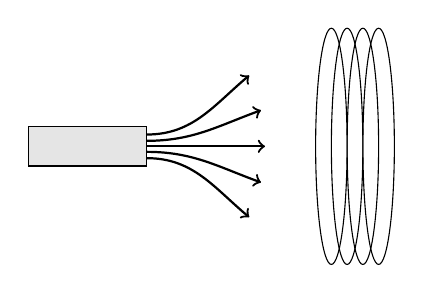
\begin{tikzpicture}
        %% Loops
        \foreach \i in {1mm,3mm,5mm,7mm} {
            \draw (\i,0) circle (0.2cm and 1.5cm);
        }
        %% magnet
        \node[draw,fill=white!90!black,minimum width=1.5cm,minimum height=0.5cm,anchor=center] (M) at (-3,0) {};
        \draw[thick,->] (M.east) ++(0,+0.15) to[out=0,in=220]  ++(30:1.5);
        \draw[thick,->] (M.east) ++(0,+0.07) to[out=0,in=200]  ++(15:1.5);
        \draw[thick,->] (M.east) to[out=0,in=180]  ++(0:1.5);
        \draw[thick,->] (M.east) ++(0,-0.07) to[out=0,in=160]  ++(-15:1.5);
        \draw[thick,->] (M.east) ++(0,-0.15) to[out=0,in=140]  ++(-30:1.5);
    \end{tikzpicture}
    \end{center}
    Which of the following would induce an emf in the coil?
    \begin{choices}
      \correctchoice{Moving the magnet toward the coil.}
      \correctchoice{Moving the coil away from the magnet.}
      \correctchoice{Turning the coil about a vertical axis.}
        %% A. I only B. II only C. I & II D. I & III E. I, II, III
    \end{choices}
\end{questionmult}
}


%% PhysicsOlympiad 1996
%%----------------------------------------
\element{aapt}{ %% Olympiad-D5
\begin{question}{olympiad-1996-q30}
    A long cylindrical conducting wire---shown in cross section below---carries a conventional current out of the page. 
    \begin{center}
    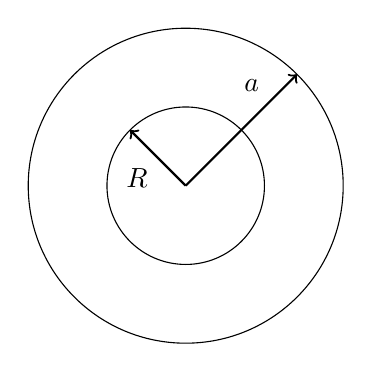
\begin{tikzpicture}
        %% cylindrical a and R
        \draw (0,0) circle (2cm);
        \draw (0,0) circle (1cm);
        %% radius a and R
        \draw[thick,->] (0,0) -- ++(45:2) node[pos=0.75,anchor=south east] {$a$};
        \draw[thick,->] (0,0) -- ++(135:1) node[pos=0.5,anchor=north east] {$R$};
    \end{tikzpicture}
    \end{center}
    The wire has uniform current density $J$ and radius $a$. 
    What is the magnetic field inside the wire,
        a distance $R$ ($R<a$) from the wire's center?
    \begin{choices}
        \wrongchoice{$\dfrac{\mu_0 J a}{2}$ clockwise}
        \wrongchoice{$\dfrac{\mu_0 J a^2}{2R}$ clockwise}
      \correctchoice{$\dfrac{\mu_0 J R}{2}$ counterclockwise}
        \wrongchoice{$\dfrac{\mu_0 J a^2}{2R}$ counterclockwise}
        \wrongchoice{$\dfrac{\mu_0 J a}{2}$ counterclockwise}
    \end{choices}
\end{question}
}


%% PhysicsOlympiad 1995
%%----------------------------------------
\element{aapt}{ %% Olympiad-D5
\begin{question}{olympiad-1995-q30}
    Identical currents flow in two perpendicular wires,
        as shown in the accompanying figure.
    The wires are very close but do not touch.
    \begin{center}
    \begin{circuitikz}[scale=0.8]
        \draw[very thick] (3,0) to (0,0) to [short,i=$I$] (-3,0);
        \draw[very thick] (0,-3) to (0,0) to [short,i=$I$] (0,3);
        \node[anchor=center] at (+1.5,+1.5) {1};
        \node[anchor=center] at (-1.5,+1.5) {2};
        \node[anchor=center] at (-1.5,-1.5) {3};
        \node[anchor=center] at (+1.5,-1.5) {4};
    \end{circuitikz}
    \end{center}
    The magnetic field can be zero:
    \begin{choices}
        \wrongchoice{at a point in region 1 only}
        \wrongchoice{at a point in region 2 only}
        \wrongchoice{at points in both regions 1 and 2}
        \wrongchoice{at points in both regions 1 and 4}
      \correctchoice{at points in both regions 2 and 4}
    \end{choices}
\end{question}
}


%% PhysicsOlympiad 1994
%%----------------------------------------
\element{aapt}{ %% Olympiad-D5
\begin{question}{olympiad-1994-q29}
    The infinitely long straight wire carries a conventional current $I$ as shown in the accompanying figure.
    The rectangular loop carries a conventional current $I^{\prime}$ in the counterclockwise direction.
    \begin{center}
    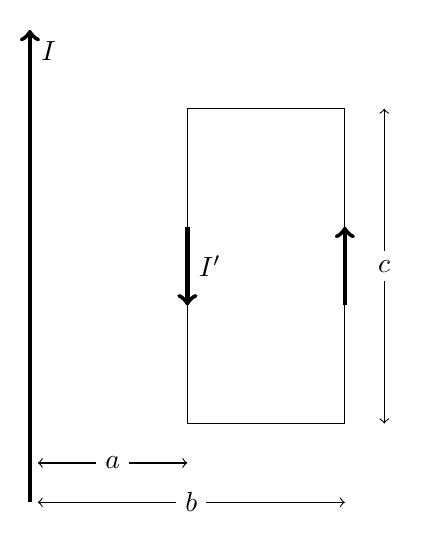
\begin{tikzpicture}
        %% Straight Wire
        \draw[ultra thick,->] (0,-3) -- (0,3) node[anchor=north west] {$I$};
        %% Wire loop
        \draw (2,-2) rectangle (4,+2);
        \draw[ultra thick,->] (2,+0.5) -- (2,-0.5) node[pos=0.5,anchor=west] {$I^{\prime}$};
        \draw[ultra thick,->] (4,-0.5) -- (4,+0.5);
        %% lengths
        \draw[<->] (4.5,-2) -- (4.5,+2) node[pos=0.5,anchor=center,fill=white] {$c$};
        \draw[<->] (0.1,-2.5) -- (2,-2.5) node[pos=0.5,anchor=center,fill=white] {$a$};
        \draw[<->] (0.1,-3) -- (4,-3) node[pos=0.5,anchor=center,fill=white] {$b$};
    \end{tikzpicture}
    \end{center}
    The net force on the rectangular loop is:
    \begin{choices}
      \correctchoice{$\dfrac{\mu II^{\prime} c}{2\pi}\left(\dfrac{1}{a}-\dfrac{1}{b}\right)$ to the right}
        \wrongchoice{$\dfrac{\mu II^{\prime} c}{2\pi}\left(\dfrac{1}{a}+\dfrac{1}{b}\right)$ to the left}
        \wrongchoice{$\dfrac{\mu II^{\prime} c}{2\pi}\left(\dfrac{c}{a}+\dfrac{c}{b}+\dfrac{2\left(b-a\right)}{c}\right)$ to the left}
        \wrongchoice{$\dfrac{\mu II^{\prime} c}{2\pi}\dfrac{2\left(a-b\right)}{c}$ to the right}
        \wrongchoice{zero}
    \end{choices}
\end{question}
}

\element{aapt}{ %% Olympiad-D5
\begin{question}{olympiad-1994-q30}
    A spatially uniform magnetic field of \SI{0.080}{\tesla} is directed into the plane of the page and perpendicular to it,
        as shown in the accompanying figure.
    A wire loop in the plane of the page has constant area \SI{0.010}{\meter\squared}.
    \begin{center}
    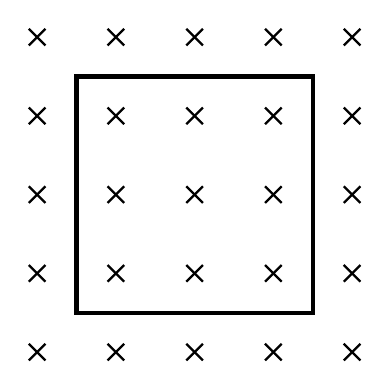
\begin{tikzpicture}
        %% B field into page
        \foreach \x in {1,2,3,4,5}
            \foreach \y in {1,2,3,4,5} {
                \draw[thick] (\x,\y) -- ++(45:0.15);
                \draw[thick] (\x,\y) -- ++(135:0.15);
                \draw[thick] (\x,\y) -- ++(225:0.15);
                \draw[thick] (\x,\y) -- ++(315:0.15);
            }
        %% Wire loop
        \draw[ultra thick] (1.5,1.5) rectangle (4.5,4.5);
    \end{tikzpicture}
    \end{center}
    The magnitude of the magnetic field decreases at a constant rate of \SI{3.0e-4}{\tesla\per\second}.
    What is the magnitude and direction of the induced emf?
    \begin{choices}
      \correctchoice{\SI{3.0e-6}{\volt} clockwise}
        \wrongchoice{\SI{3.0e-6}{\volt} counterclockwise}
        \wrongchoice{\SI{2.4e-5}{\volt} counterclockwise}
        \wrongchoice{\SI{8.0e-4}{\volt} counterclockwise}
        \wrongchoice{\SI{8.0e-4}{\volt} clockwise}
    \end{choices}
\end{question}
}



\endinput


